
% ----------------------------------------------------------------------
%  Set the document class
% ----------------------------------------------------------------------
\documentclass[11pt,a4paper,twoside]{article}

% ----------------------------------------------------------------------
% Define external packages, language, margins, fonts and new commands
% ----------------------------------------------------------------------
%\input{preamble} 
\usepackage[utf8]{inputenc}   % <<<<< Linux
\usepackage[english]{babel} % <<<<< English
\usepackage{notoccite}
\usepackage[skip=0.5\baselineskip]{caption}
\hyphenation{GTKWave}
\usepackage{listings}
\usepackage[all]{nowidow}

%blind text
\usepackage{lipsum}

\usepackage{graphicx}
\graphicspath{ {./} {../../figlib/} }
\def\FontLn{% 16 pt normal
  \usefont{T1}{phv}{m}{n}\fontsize{16pt}{16pt}\selectfont}
\def\FontLb{% 16 pt bold
  \usefont{T1}{phv}{b}{n}\fontsize{16pt}{16pt}\selectfont}
\def\FontMn{% 14 pt normal
  \usefont{T1}{phv}{m}{n}\fontsize{14pt}{14pt}\selectfont}
\def\FontMb{% 14 pt bold
  \usefont{T1}{phv}{b}{n}\fontsize{14pt}{14pt}\selectfont}
\def\FontSn{% 12 pt normal
  \usefont{T1}{phv}{m}{n}\fontsize{12pt}{12pt}\selectfont}

% Use Arial font as default
%
\renewcommand{\rmdefault}{phv}
\renewcommand{\sfdefault}{phv}
\usepackage{geometry}	
\geometry{verbose,tmargin=2.5cm,bmargin=2.5cm,lmargin=2.5cm,rmargin=2.5cm}

%\usepackage{setspace}
%\renewcommand{\baselinestretch}{1.5}

\usepackage[pdftex]{hyperref} % enhance documents that are to be
                              % output as HTML and PDF
\hypersetup{colorlinks,       % color text of links and anchors,
                              % eliminates borders around links
%            linkcolor=red,    % color for normal internal links
            linkcolor=black,  % color for normal internal links
            anchorcolor=black,% color for anchor text
%            citecolor=green,  % color for bibliographical citations
            citecolor=black,  % color for bibliographical citations
%            filecolor=magenta,% color for URLs which open local files
            filecolor=black,  % color for URLs which open local files
%            menucolor=red,    % color for Acrobat menu items
            menucolor=black,  % color for Acrobat menu items
%            pagecolor=red,    % color for links to other pages
            pagecolor=black,  % color for links to other pages
%            urlcolor=cyan,    % color for linked URLs
            urlcolor=black,   % color for linked URLs
	          bookmarks=true,         % create PDF bookmarks
	          bookmarksopen=false,    % don't expand bookmarks
	          bookmarksnumbered=true, % number bookmarks
	          pdftitle={report},
            pdfauthor={Andre C. Marta},
%            pdfsubject={Thesis Title},
%            pdfkeywords={Thesis Keywords},
            pdfstartview=FitV,
            pdfdisplaydoctitle=true}

\usepackage[numbers,sort&compress]{natbib} % <<<<< References in numbered list [1],[2],...
\usepackage{subcaption} 
\usepackage{mdframed}

%%%%%%%%%%%%%%%%%%%%%%%%%%%%%%%%%%%%%%%%%%%%%%%%%%%%%%%%%%%%%%%%%%%%%%%%
%     Begin Document                                                   %
%%%%%%%%%%%%%%%%%%%%%%%%%%%%%%%%%%%%%%%%%%%%%%%%%%%%%%%%%%%%%%%%%%%%%%%%


\begin{document}

% Set plain page style (no headers, footer with centered page number)
\pagestyle{plain}

% Set roman numbering (i,ii,...) before the start of chapters
%\pagenumbering{roman}

% ----------------------------------------------------------------------
%  Cover page
% ----------------------------------------------------------------------
%%%%%%%%%%%%%%%%%%%%%%%%%%%%%%%%%%%%%%%%%%%%%%%%%%%%%%%%%%%%%%%%%%%%%%%%
%                                                                      %
%     File: Thesis_FrontCover.tex                                      %
%     Tex Master: Thesis.tex                                           %
%                                                                      %
%     Author: Andre C. Marta                                           %
%     Last modified :  2 Jul 2015                                      %
%                                                                      %
%%%%%%%%%%%%%%%%%%%%%%%%%%%%%%%%%%%%%%%%%%%%%%%%%%%%%%%%%%%%%%%%%%%%%%%%

\thispagestyle {empty}

% IST Logo - Signature A
% parameters: bb=llx lly urx ury (bounding box), width=h_length, height=v_length, angle=angle, scale=factor, clip=true/false, draft=true/false. 
\includegraphics[bb=9.5cm 11cm 0cm 0cm,scale=0.29]{IST_A_CMYK_POS}

\begin{center}
%
% Figure (Image or plot)
\vspace{1.0cm}
% height = 50 mm
%\includegraphics[height=50mm]{Figures/Airbus_A350.jpg}

% Title, author and degree
\vspace{1cm}
{\FontLb Circuit Theory and Electronics Fundamentals} \\ % <<<<< EDIT TITLE
\vspace{1cm}
{\FontSn Department of Electrical and Computer Engineering, Técnico, University of Lisbon} \\ % <<<<< EDIT COURSE
\vspace{1cm}
{\FontSn Laboratory Two Report} \\
\vspace{1cm}
{\FontSn Francisco Batista, 95792.} \\
{\FontSn Miguel Jesus, 95833.} \\
{\FontSn Pedro Monteiro, 96465.} \\
\vspace{1cm}
{\FontSn April 5, 2021} \\ % <<<<< EDIT DATE (corresponds to date of oral examination)
%
\end{center}



% ----------------------------------------------------------------------
% Dedication page (optional)
% ----------------------------------------------------------------------
%\input{dedication} 
%\cleardoublepage

% ----------------------------------------------------------------------
%  Acknowledgments (optional)
% ----------------------------------------------------------------------
%\input{acknowledgements}
%\cleardoublepage

% ----------------------------------------------------------------------
%  Abstract (both in English and Portuguese)
% ----------------------------------------------------------------------
%\input{resumo} 
%\cleardoublepage

%\input{abstract} 

% ----------------------------------------------------------------------
%  Table of contents, list of tables, list of figures and nomenclature
% ----------------------------------------------------------------------

% Table of contents

\vspace{8.5cm}

\tableofcontents

% List of tables
%\addcontentsline{toc}{section}{\listtablename}
%\listoftables
%\cleardoublepage 

% List of figures
%\addcontentsline{toc}{section}{\listfigurename}
%\listoffigures
%\cleardoublepage 

% Set arabic numbering (1,2,...) after preface
%
%\setcounter{page}{1}
%\pagenumbering{arabic}

% ----------------------------------------------------------------------
%  Body
% ----------------------------------------------------------------------


\section{Introduction}
\label{sec:introduction}

% state the learning objective 
The objective of this laboratory assignment is create an AC/DC converter circuit using an envelope detector and a voltage regulator with an architecture decided by the students. To do so we created the circuit presented below. In the circuit it can be identified a full wave rectifier that is used in order to achieve DC voltage. Then we use a capacitor to estabilize the voltage value. Finally the use of a voltage regulator that allow us to obtain a constant output voltage value of 12 Volts. The theoretical analysis was made using the Octave toll and for the simulation analysis we used the Ngspice Software.





\section{Theoretical Analysis}
\label{sec:analysis}

In this section, the circuit shown in Figure~\ref{fig:T2Circuit} is analysed theoretically in six steps.

In step (1), first of all, we used the nodal method to determine the voltages in all nodes and currents in all branches for t<0. The results are shown in Table~\ref{tab:TA1}.

\begin{table}[h]
  \centering
  \begin{tabular}{|l|r|}
    \hline    
    {\bf Nodes and branches} & {\bf Value [V]/[A]} \\ \hline
    v1 & 5.134164 \\ \hline
v2 & 4.929601 \\ \hline
v3 & 4.510168 \\ \hline
v4 & 0.000000 \\ \hline
v5 & 4.957651 \\ \hline
v6 & 5.588276 \\ \hline
v7 & -2.095712 \\ \hline
v8 & -3.151534 \\ \hline
  \end{tabular}
  \caption{Theoretical voltage values for each node, expressed in Volt, and current values for each branch, expressed in Ampere.}
  \label{tab:TA1}
\end{table}

After this, in step (2), we determined the equivalent resistance as seen from the capacitor terminals. In order to do so, we followed the professor's sugestion. Therefore, in this section of the analysis, the capacitor was replaced by a voltage source Vx. Ix and Vx were calculated using Octave. After this, the value of the equivalent resistance was computed and determined. These procedures were necessary because they allowed us to calculate the time constant (\tau) without which we would no be able to performe all the theoretical analisys in the following sections. 

\begin{equation}
  \tau = R_{eq}C,
  \label{eq:tau}
\end{equation}


The computed results can be found in Table~\ref{tab:TA2}.

\begin{table}[h]
  \centering
  \begin{tabular}{|l|r|}
    \hline    
    {\bf Computed Results} & {\bf Values} \\ \hline
    v1 & 0.000000 \\ \hline
v2 & 0.000000 \\ \hline
v3 & 0.000000 \\ \hline
v4 & 0.000000 \\ \hline
v5 & 0.000000 \\ \hline
v6 & 8.739810 \\ \hline
v7 & 0.000000 \\ \hline
v8 & 0.000000 \\ \hline
Ix & -0.002826 \\ \hline
Vx & 8.739810 \\ \hline
Req & -3092.796241 \\ \hline
  \end{tabular}
  \caption{Computed results: voltage expressed in Volt, current in Ampere and resistence in Ohm.}
  \label{tab:TA2}
\end{table}

Later, in step (3), we used the value of the equivalent resistant calculated in point (2) to find the natural solution of v6. Knowing that "\tau" is calculated by the equation~\ref{tau}, in Equation~\ref{eq:natsol} we find the formula required to calculate the natural solution we wanted. 

\begin{equation}
  V_{6n}(t) = V_{x}e^{-\frac{t}{\tau}},
  \label{eq:natsol}
\end{equation}

Also the solution is ploted in Figure~\ref{figure:plotA(4)} where the x-axis corresponds to time, t, expressed in [ms] and the y-axis corresponds to the natural solution of v6, 'v6n', expressed in [V].

\begin{figure}[h] \centering
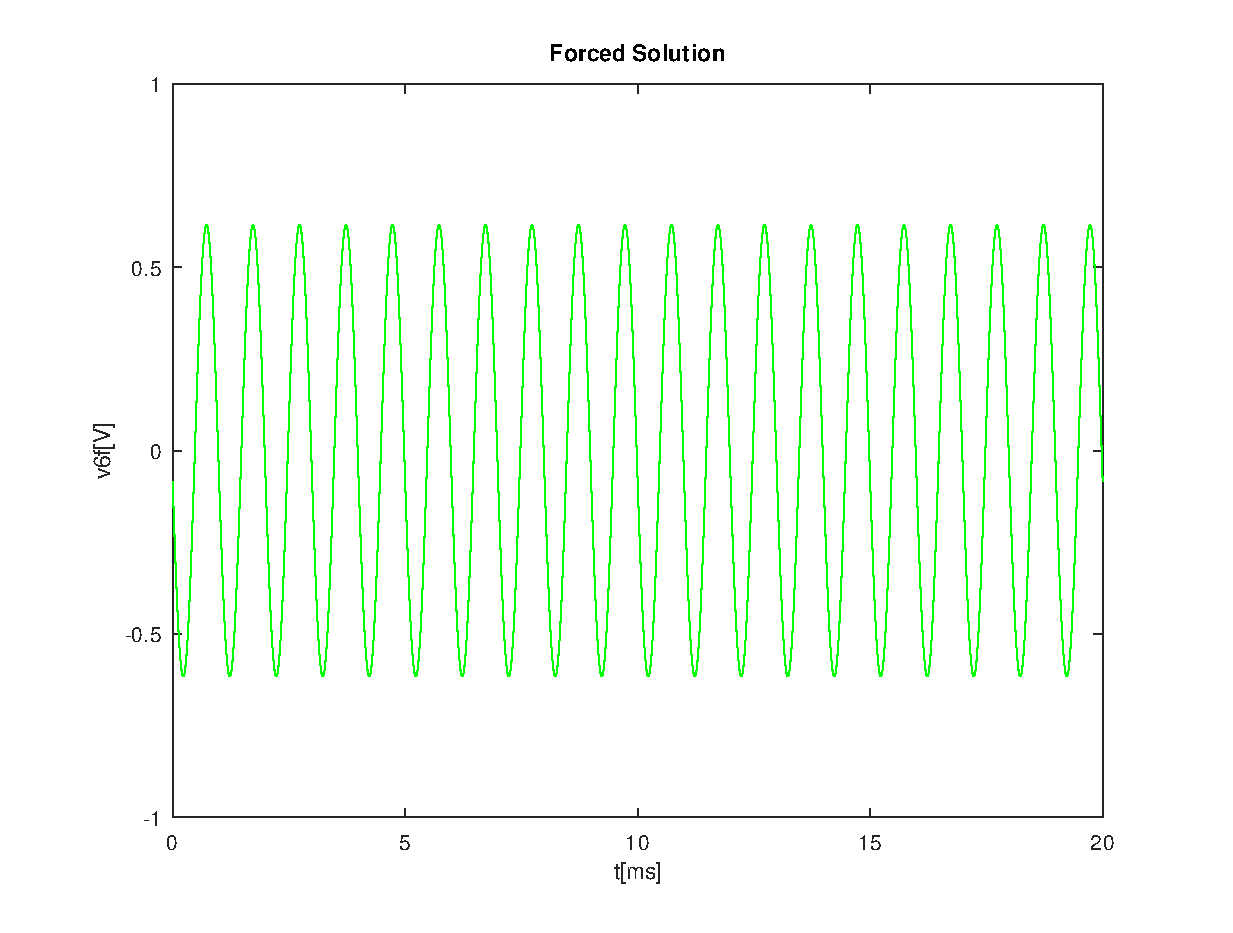
\includegraphics[width=0.8\linewidth]{forced_solution.eps}
\caption{Plot of v6n(t) in the interval [0, 20]ms.}
\label{fig:plotA(4)}
\end{figure}

In step (4), the forced solution v6f(t) was determined for f=1KHz and for t in the interval [0,20]ms. Moreover, the capacitance was replaced by the impedance, 'Z', and Vs was considered equal to one. The complex amplitudes in the nodes are shown in Table~\ref{tab:TA4}.

\begin{table}[h]
  \centering
  \begin{tabular}{|l|r|}
    \hline    
    {\bf Nodes} & {\bf Complex Amplitudes} \\ \hline
    |v1| & 1.000000 \\ \hline
|v2| & 0.960156 \\ \hline
|v3| & 0.878462 \\ \hline
|v4| & 0.000000 \\ \hline
|v5| & 0.965620 \\ \hline
|v6| & -0.609606 \\ \hline
|v7| & -0.408190 \\ \hline
|v8| & -0.613836 \\ \hline
  \end{tabular}
  \caption{Complex amplitudes in the nodes, expressed in Volt.}
  \label{tab:TA4}
\end{table}

Then, in step (5), we determined the final total solution v6(t) by converting the phasors to real time functions for f=1KHz, and superimposing the natural and forced solutions, just like it was asked by the professor. In Figure~\ref{fig:plotA(5)} are plotted both vs(t) and v6(t) in the interval [-5, 20]ms.

\begin{figure}[h] \centering
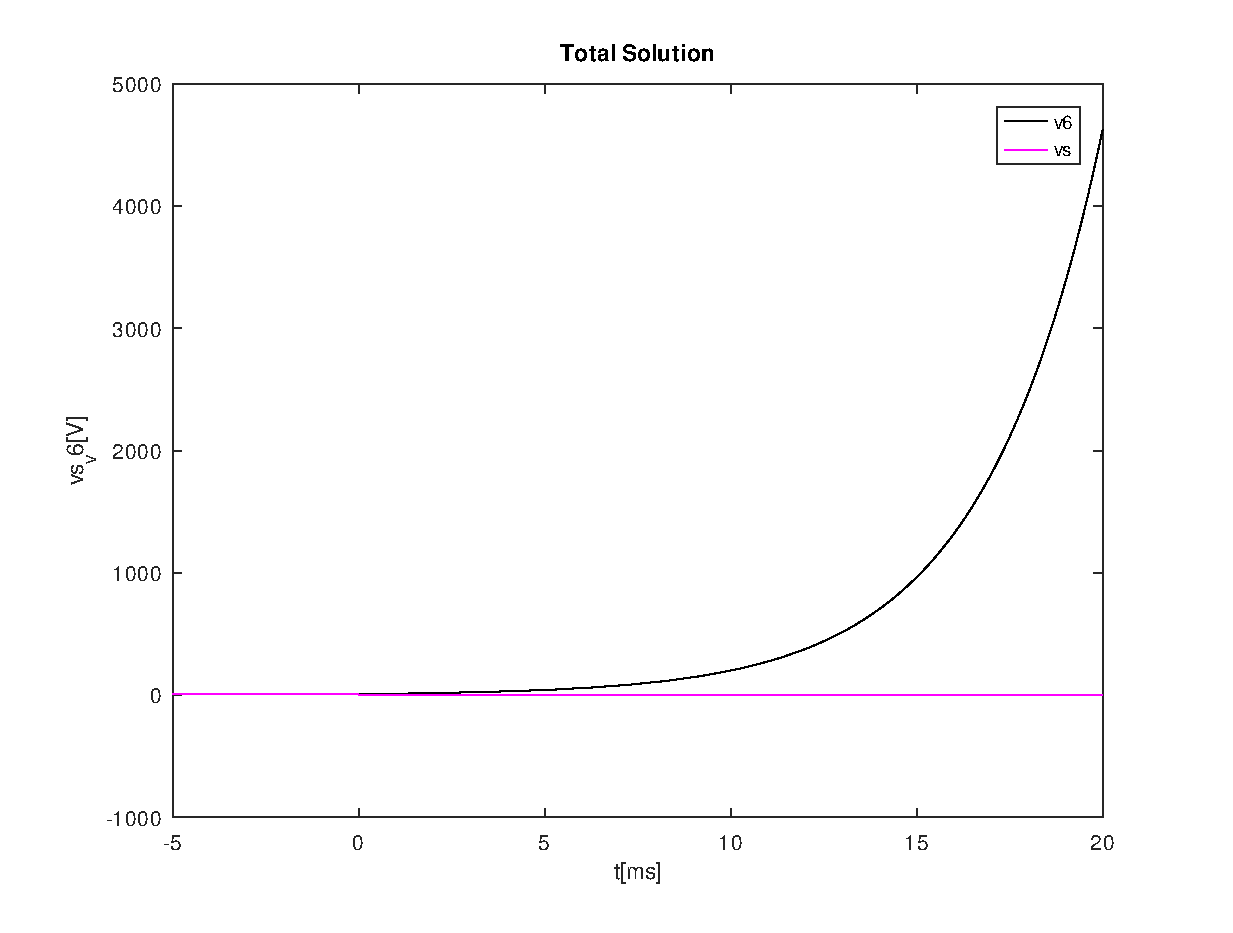
\includegraphics[width=0.8\linewidth]{Total_Solution.eps}
\caption{Plot of v6(t) and vs(t) in the interval [-5, 20]ms.}
\label{fig:plotA(5)}
\end{figure}

Finally, in step (6), we calculted the frequency responses vc(f) and v6(f) for frequency in the interval [0.1, 1M]Hz. The functions vs(f), vc(f) and v6(f) are represented in two plots: one of amplitude frequency response, represented in Figure~\ref{fig:plotA(61)} and the other of phase response, shown in Figure~\ref{fig:plotA(62)}. Note that in both graphs, frequency logscale magnitude is in dB and phase in degrees.

\begin{figure}[h] \centering
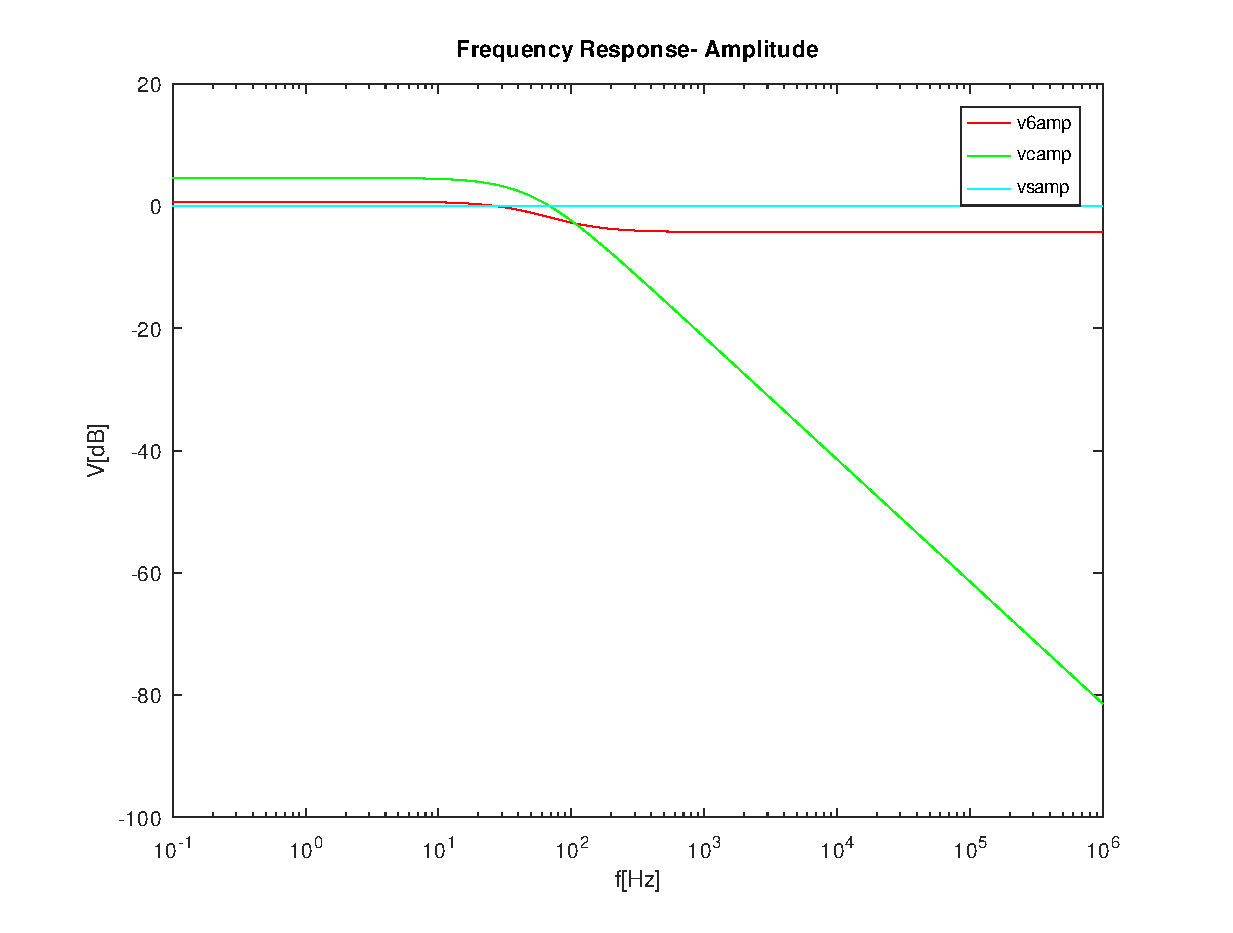
\includegraphics[width=0.8\linewidth]{Frequency_Response_Amplitude.eps}
\caption{Plot of amplitude frequency response (for vs(f), vc(f) and v6(f)) in the interval [0.1, 1M]Hz.}
\label{fig:plotA(61)}
\end{figure}

\begin{figure}[h] \centering
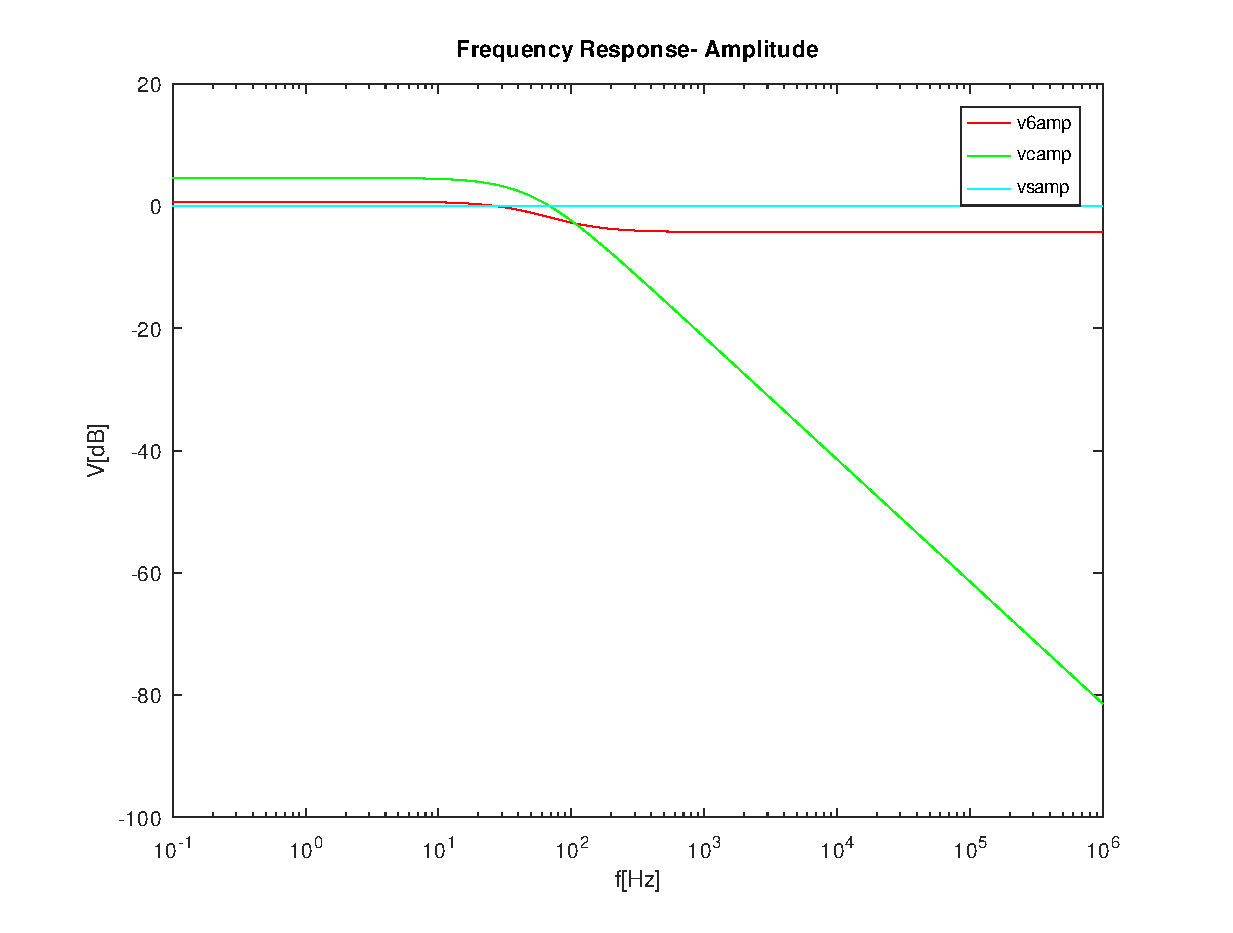
\includegraphics[width=0.8\linewidth]{Frequency_Response_Phase.eps}
\caption{Plot of phase response (for vs(f), vc(f) and v6(f)) in the interval [0.1, 1M]Hz.}
\label{fig:plotA(62)}
\end{figure}

How and why they differ??....


\section{Simulation Analysis}
\label{sec:simulation}

\subsection{Operating Point Analysis}

Following our theoretical analysis, the circuit was simulated in the Ngspice software, which returned the values of the voltage for each node. These values, that are shown in Table~\ref{tab:op}, allowed us to easily calculate the electrical currents. 
The inputs given to the Ngspice were the values of the resistors, as well as the nodes to which they are connected (the positive being followed by the negative), and their values. Moreover, the independent current and voltage source, as well as the values for K_b and K_c, which are fundamental to the controlled sources, are also introduced. 
In order for the current that commands the controlled voltage to flow from the positive to the negative node, the creation of a control, ficticious node was necessary to sense this current.
When compared, the results of the theoretical analysis and the simulated ones are approximately the same, with tiny differences that might be owed to factors such as Octave rounding errors in the matrix equations.

\begin{table}[h]
  \centering
  \begin{tabular}{|l|r|}
    \hline    
    {\bf Name} & {\bf Value [A or V]} \\ \hline
    @cb[i] & 0.000000e+00\\ \hline
@ce[i] & 0.000000e+00\\ \hline
@q1[ib] & 7.022567e-05\\ \hline
@q1[ic] & 1.404513e-02\\ \hline
@q1[ie] & -1.41154e-02\\ \hline
@q1[is] & 5.765392e-12\\ \hline
@rc[i] & 1.411536e-02\\ \hline
@re[i] & 1.411536e-02\\ \hline
@rf[i] & 7.022567e-05\\ \hline
@rs[i] & 0.000000e+00\\ \hline
v(1) & 0.000000e+00\\ \hline
v(2) & 0.000000e+00\\ \hline
base & 2.254108e+00\\ \hline
coll & 5.765392e+00\\ \hline
emit & 1.411536e+00\\ \hline
vcc & 1.000000e+01\\ \hline

  \end{tabular}
  \caption{Operating point. Simulated Values for voltage (V) and current (A) using Ngspice.}
  \label{tab:op}
\end{table}






\newpage

\section{Conclusion}
\label{sec:conclusion}

To sum up, in this assignment, the main goal was successfully achieved. This objective was to analyze a circuit with varius components such as resistors, a voltage source that changes over time and a capacitor.

To perform this study we used the Octave and Ngspice tools for the theoretical and simulation analysis, respectively.

The values that were obtained in both analysis are very similar. nevertheless, there are small discrepancies between the sets of values. These differences are due to approximations, made particularly by Ngspice, as this software has a different level of digit precision when compared to Octave. Whereas some values in Octave are presented as 0, in Ngspice the same values are simulated with the order of 1e-14 or 1e-15 which we can consider to be also zero. Therefore the relative error between the theoretical and simulated results are very close to 0\%.

The proximity between the values obtained in the static, time and frequency analysis in the theoretical and simulation section can be explained with the simplicity of the circuit that is only made of linear components and one capacitor.


%\cleardoublepage

% ----------------------------------------------------------------------
%  Bibliography
% ----------------------------------------------------------------------
%\addcontentsline{toc}{section}{\bibname}
%\bibliographystyle{abbrvunsrtnat} % <<<<< SELECT IF USING REFERENCES BY NUMBER (CITATION ORDER)
%\bibliography{../../../BIBfile.bib}

% ----------------------------------------------------------------------
\end{document}
% ----------------------------------------------------------------------

